\documentclass[11pt,a4paper]{article}
\usepackage[T1]{fontenc}
\usepackage[utf8]{inputenc}
\usepackage{lmodern,amsmath,amssymb,amsthm,mathtools}
\usepackage[margin=27mm]{geometry}
\usepackage{booktabs,array,longtable,microtype,xcolor,tikz,listings}
\usepackage[colorlinks=true,linkcolor=blue!45!black,citecolor=blue!45!black,urlcolor=blue!45!black]{hyperref}
\usepackage{fancyhdr}
\hypersetup{pdftitle={A Seven-Coefficient Obstruction to Wagner's Forest Sum-of-Squares Conjecture},pdfauthor={Research draft prepared for Keio},pdfsubject={Exact obstruction to a prescribed forest sum-of-squares identity}}
\pagestyle{fancy}\fancyhf{}
\fancyhead[L]{\small A forest sum-of-squares obstruction}
\fancyhead[R]{\small Research draft}
\fancyfoot[C]{\thepage}
\setlength{\headheight}{14pt}
\setlength{\parskip}{4pt}
\setlength{\parindent}{0pt}
\newtheorem{theorem}{Theorem}
\newtheorem{lemma}[theorem]{Lemma}
\newtheorem{corollary}[theorem]{Corollary}
\newtheorem{proposition}[theorem]{Proposition}
\newcommand{\FF}{\mathcal F}
\newcommand{\SSS}{\mathcal S}
\newcommand{\Asets}{\mathcal A}
\newcommand{\ind}{\mathbf 1}
\newcommand{\R}{\mathbb R}
\newcommand{\Z}{\mathbb Z}
\newcommand{\Ftwo}{\mathbb F_2}
\newcommand{\coef}[2]{[\boldsymbol y^{#1}]#2}
\lstset{language=Python,basicstyle=\ttfamily\scriptsize,
  keywordstyle=\color{blue!50!black},commentstyle=\color{black!55},
  stringstyle=\color{green!35!black},breaklines=true,breakatwhitespace=false,
  columns=fullflexible,keepspaces=true,showstringspaces=false,
  frame=single,rulecolor=\color{black!15},numbers=left,
  numberstyle=\tiny\color{black!45},numbersep=7pt,xleftmargin=13pt,
  aboveskip=9pt,belowskip=9pt}
\title{A Seven-Coefficient Obstruction to Wagner's\newline
Forest Sum-of-Squares Conjecture}
\author{Research draft prepared for Keio}
\date{November 2026}

\begin{document}
\maketitle
\begin{abstract}
We give an exact obstruction to the prescribed signed sum-of-squares
identity in Conjecture~1.3 of Erickson (2012), attributed there to
Wagner. The graph is the eight-vertex M\"obius ladder, and the two
distinguished edges are opposite edges of its outer cycle. Seven
coefficients of the proposed identity force two signs $T,U\in\{-1,1\}$
to satisfy $T+4U=4$, an impossibility. The proof excludes every sign
assignment, without a numerical tolerance or an unproved auxiliary
assumption. A second seven-coefficient argument excludes even multiple
polynomial squares with arbitrary real coefficients on the prescribed
monomial supports. Edge deletion excludes the original identity on every
complete graph $K_n$ with $n\ge8$. We also explain a general reduction
of such sign identities to linear equations over $\Ftwo$ by working
modulo~$8$. The same Rayleigh difference nevertheless has an explicit
unrestricted monomial-times-squares representation, giving a strict
separation between the prescribed supports and general square certificates.
The forest negative-correlation conjecture is not refuted. The source explicitly
reports a private verification for the M\"obius ladder; our coefficient
certificate conflicts with that report. The full finite verification
is therefore included, and no historical-priority claim is made.
\end{abstract}

\section{The exact previously stated conjecture}

For a finite simple graph $G=(V,E)$, let
\[
 F_G(\boldsymbol y)=\sum_{X\in\FF(G)}\boldsymbol y^X,
 \qquad \boldsymbol y^X=\prod_{g\in X}y_g,
\]
where $\FF(G)$ consists of \emph{all} acyclic edge subsets, including
the empty set. The associated forest Rayleigh difference at distinct
edges $e,f$ is
\begin{equation}\label{eq:rayleigh}
 \Delta_{G,e,f}=(\partial_eF_G)(\partial_fF_G)
                  -F_G\partial_e\partial_fF_G.
\end{equation}
Writing $F_G=Z+y_eA+y_fB+y_ey_fC$ shows directly that
$\Delta_{G,e,f}=AB-ZC$ is independent of $y_e,y_f$.
The symbols $A,B,C$ in this decomposition are used only in this paragraph.

The weighted forest negative-correlation conjecture asserts
$\Delta_{G,e,f}(\boldsymbol y)\ge0$ for positive weights. The relevant
conjecture in this paper is the \emph{specified signed polynomial
identity} proposed as a sufficient explanation of that inequality.
We use precisely Definition~1.2 and Conjecture~1.3 of
Erickson~\cite{Erickson2012}.

Let $H=E\setminus\{e,f\}$ and set
\[
 \SSS=\{S\subseteq H:S\cup\{e,f\}\text{ is contained in a simple cycle of }G\}.
\]
For $S\in\SSS$, let $\Asets(S)$ consist of forests $A\subseteq H$ such
that $A\cup\{e,f\}$ has exactly one cycle $C_A$, with
$S\cup\{e,f\}\subseteq C_A$. For each admissible pair $(S,C)$ choose
a sign $c(S,C)\in\{-1,1\}$, shared by all forests having the same
$S$ and the same cycle. The conjectured identity is
\begin{equation}\label{eq:wagner}
 \Delta_{G,e,f}
 =R_c(\boldsymbol y):=
 \sum_{S\in\SSS}\boldsymbol y^S
 \left(\sum_{A\in\Asets(S)}c(S,C_A)\boldsymbol y^{A\setminus S}\right)^2.
\end{equation}
The quantifier is that for \emph{every} graph and \emph{every} pair
of distinct edges, some choice of these signs makes the identity hold.
An earlier public statement is Conjecture~5.2.6 of Erickson's
2008 thesis~\cite{Erickson2008}.

\begin{theorem}\label{thm:main}
Let $M_8$ be the graph with vertex set $\{0,1,\ldots,7\}$, outer
cycle edges $\{i,i+1\pmod8\}$, and opposite chords $\{i,i+4\}$
for $0\le i\le3$. Take $e=01$ and $f=45$.
There is no sign assignment $c(S,C)\in\{-1,1\}$ satisfying
\eqref{eq:wagner}. Consequently, the universal assertion in
\cite[Conjecture~1.3]{Erickson2012} is false as stated.
\end{theorem}

Here and below $uv$ denotes the unordered edge $\{u,v\}$. This is a
statement about equality of polynomials, with the original graph,
forest sets, cycles, exponents, and signs of the conjecture.

\section{The graph and the seven coefficient equations}

Order the ten unmarked edges as
\begin{equation}\label{eq:edgeorder}
 (h_1,\ldots,h_{10})=(04,07,12,15,23,26,34,37,56,67).
\end{equation}
Figure~\ref{fig:graph} displays the graph. The edge order in
\eqref{eq:edgeorder}, rather than the drawing, specifies the certificate.

\begin{figure}[ht]
\centering
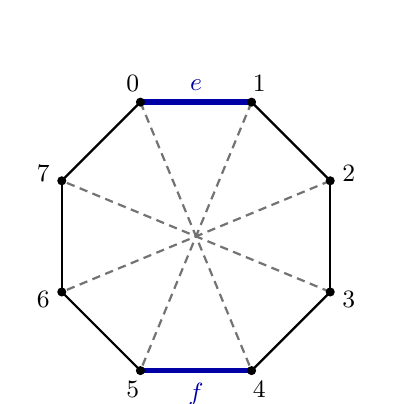
\begin{tikzpicture}[scale=.82,every node/.style={font=\small}]
 \foreach \i in {0,...,7}{
   \coordinate (v\i) at ({112.5-45*\i}:2.25);
 }
 \foreach \i/\j in {0/1,1/2,2/3,3/4,4/5,5/6,6/7,7/0}
   \draw[line width=.8pt] (v\i)--(v\j);
 \foreach \i/\j in {0/4,1/5,2/6,3/7}
   \draw[densely dashed,black!55,line width=.8pt] (v\i)--(v\j);
 \draw[blue!65!black,line width=2.1pt] (v0)--node[above]{$e$}(v1);
 \draw[blue!65!black,line width=2.1pt] (v4)--node[below]{$f$}(v5);
 \foreach \i in {0,...,7}{
   \fill (v\i) circle(2pt);
   \node at ({112.5-45*\i}:2.56){\i};
 }
\end{tikzpicture}
\caption{The eight-vertex M\"obius ladder. Dashed lines are edges;
their interior intersections are not vertices. The marked edges
are opposite outer-cycle edges.}\label{fig:graph}
\end{figure}

For a nonnegative integer mask $b<2^{10}$, write
$H_b=\{h_j:\text{bit }j-1\text{ of }b\text{ is }1\}$.
This notation is only an exact encoding of subsets. Put
\[
 c_{s,b}=c(H_s,H_b\cup\{e,f\}).
\]
The seven cycle masks occurring in the proof are listed in
Table~\ref{tab:cycles}. Each listed edge set becomes a simple cycle
when $e$ and $f$ are added.

\begin{table}[ht]
\centering
\begin{tabular}{rll}
\toprule
$b$ & Indices $j$ with $h_j\in H_b$ & A cyclic vertex order \\
\midrule
9   & $1,4$             & $0,1,5,4,0$\\
202 & $2,4,7,8$         & $0,1,5,4,3,7,0$\\
293 & $1,3,6,9$         & $0,1,2,6,5,4,0$\\
486 & $2,3,6,7,8,9$     & $0,1,2,6,5,4,3,7,0$\\
634 & $2,4,5,6,7,10$    & $0,1,5,4,3,2,6,7,0$\\
854 & $2,3,5,7,9,10$    & $0,1,2,3,4,5,6,7,0$\\
917 & $1,3,5,8,9,10$    & $0,1,2,3,7,6,5,4,0$\\
\bottomrule
\end{tabular}
\caption{The cycles used in the coefficient certificate.}\label{tab:cycles}
\end{table}

Define the following products of signs:
\begin{equation}\label{eq:products}
\begin{aligned}
 A&=c_{528,634}c_{528,854},&
 B&=c_{528,854}c_{528,917},&
 D&=c_{0,9}c_{0,854},\\
 E_*&=c_{1,9}c_{1,293},&
 F_*&=c_{8,9}c_{8,634},&
 G_*&=c_{32,293}c_{32,634},\\
 P&=c_{0,9}c_{0,486},&
 Q&=c_{1,9}c_{1,917},&
 R&=c_{128,202}c_{128,917},\\
 T&=c_{0,202}c_{0,293},&
 U&=c_{8,9}c_{8,202}.&&
\end{aligned}
\end{equation}
All of these are in $\{-1,1\}$. In addition,
\begin{equation}\label{eq:AB}
 c_{528,634}c_{528,917}=AB.
\end{equation}
The subsets indexing the signs are $H_0=\varnothing$, $H_1=\{h_1\}$,
$H_8=\{h_4\}$, $H_{32}=\{h_6\}$, $H_{128}=\{h_8\}$,
and $H_{528}=\{h_5,h_{10}\}$. Each is contained in every cycle
with which it is paired above.

For $v=(v_1,\ldots,v_{10})$, write $[v]F$ for the coefficient of
$\prod_j y_{h_j}^{v_j}$ in $F$. The following table gives five
necessary coefficient equations for \eqref{eq:wagner}.

\begin{table}[ht]
\centering\small
\begin{tabular}{clrl}
\toprule
Row & $v$ & $[v]\Delta_{M_8,e,f}$ & $[v]R_c$\\
\midrule
1 & $(0,2,1,1,1,1,2,0,1,1)$ & $-2$ & $2A$\\
2 & $(1,1,2,0,1,0,1,1,2,1)$ & $-2$ & $2B$\\
3 & $(1,1,2,1,1,1,2,0,1,2)$ & $-2$ & $2D$\\
4 & $(1,0,1,1,0,1,0,0,2,2)$ & $4$ & $2+2E_*$\\
5 & $(1,2,1,1,1,1,2,0,1,1)$ & $0$ & $2(D+E_*+F_*+G_*)$\\
\bottomrule
\end{tabular}
\caption{Five small coefficient equations.}\label{tab:small}
\end{table}

Row~6 has all ten exponents equal to $1$. Row~7 has exponent $2$
on $h_3$ and exponent $1$ on each of the other nine edges.
Their equations are
\begin{align}
74={}&28+2P+2D+8T+20E_*+2Q+20U\notag\\
     &{}+2F_*+2G_*+2R+2AB,\label{eq:row6}\\
16={}&2P+2D+4T+8E_*+2Q+4U+2R.\label{eq:row7}
\end{align}
Section~\ref{sec:verification} gives the complete finite procedure
for reproducing every coefficient, including the separate counts
in the two products defining $\Delta$.

\begin{proof}[Proof of Theorem~\ref{thm:main}]
Assume that \eqref{eq:wagner} holds. The first four rows of
Table~\ref{tab:small} force
\[
 A=B=D=-1,\qquad E_*=1.
\]
The fifth gives $F_*+G_*=0$, and \eqref{eq:AB} gives $AB=1$.
Substitution in \eqref{eq:row6} and \eqref{eq:row7} yields
\[
 P+Q+R+4T+10U=13,\qquad
 P+Q+R+2T+2U=5.
\]
Subtracting shows $2T+8U=8$, hence
\begin{equation}\label{eq:contradiction}
 \boxed{T+4U=4.}
\end{equation}
Since $T\in\{-1,1\}$ and $U$ is an integer, the left side is odd
and the right side is even. This is impossible.
\end{proof}

\section{Consequences and a general parity test}

\begin{lemma}\label{lem:deletion}
If a graph $G$ has a representation \eqref{eq:wagner} for $e,f$, so
does the graph obtained by deleting any collection of unmarked edges.
\end{lemma}
\begin{proof}
Set the weights of the deleted edges equal to zero. The forest
polynomial becomes that of the remaining graph, so the same holds
for its Rayleigh difference. On the right, a term with a deleted
edge in $S$ vanishes through $\boldsymbol y^S$. A term with a deleted
edge in $A\setminus S$ vanishes through its inner monomial. The
surviving terms are exactly the original $S$-sets and $A$-sets
for the remaining graph, with their unchanged signs. Isolated
vertices do not affect any of these polynomials or conditions.
\end{proof}

\begin{corollary}\label{cor:complete}
For every $n\ge8$, the complete graph $K_n$ does not satisfy the
universal signed identity \eqref{eq:wagner} for all pairs of edges.
More generally, any graph containing a copy of $M_8$ as a subgraph
fails that identity for a corresponding pair of opposite rim edges.
\end{corollary}
\begin{proof}
Delete all edges other than those of that copy of $M_8$, and apply
Lemma~\ref{lem:deletion} and Theorem~\ref{thm:main}.
\end{proof}
The stronger closure under minors is proved in
\cite[Lemma~2.1]{Erickson2012}; it is not needed for this corollary.

The short proof above can be found by a general, exact parity test.
For each sign write $c_v=1-2x_v$ with $x_v\in\{0,1\}$, where
$v$ denotes an admissible pair $(S,C)$. Let $R_+$ be the right
side of \eqref{eq:wagner} with all signs equal to $+1$.
An unordered pair of distinct monomials in one square contributes
$2c_vc_w$. Therefore
\begin{equation}\label{eq:mod8}
 2-2c_vc_w=4(x_v+x_w)-8x_vx_w
              \equiv4(x_v+x_w)\pmod8.
\end{equation}
If $v=w$, the product is identically $1$ and contributes no variable.

\begin{proposition}\label{prop:mod8}
For each exponent vector $\mu$, collect all unordered cross terms
of $R_c$ that contribute to that exponent. Let $L_\mu(x)$ be the
sum over $\Ftwo$ of their two sign variables, with multiplicities.
If \eqref{eq:wagner} holds, then
\[
 \coef{\mu}{(R_+-\Delta)}\equiv0\pmod4,
 \qquad
 L_\mu(x)=\frac{\coef{\mu}{(R_+-\Delta)}}4\pmod2.
\]
Any collection of these equations whose variable sides cancel and
whose right sides sum to $1$ is a complete obstruction to the
signed identity.
\end{proposition}
\begin{proof}
Expand each square and apply \eqref{eq:mod8} to its cross terms.
All diagonal terms are sign independent. The asserted equations
follow coefficient by coefficient; summing an inconsistent subset
would give $0=1$ in $\Ftwo$.
\end{proof}

For the seven rows used here, the all-positive coefficients,
in row order, are
\[
 2,\ 2,\ 2,\ 4,\ 8,\ 90,\ 24,
\]
and their sum is $132$. The corresponding coefficients of
$\Delta$ sum to $88$. The sign-variable incidences cancel over
$\Ftwo$, while $(132-88)/4=11$ is odd. The direct proof leading to
\eqref{eq:contradiction} is a hand-checkable reduction of this
parity certificate. This is an exact noncancellation obstruction,
not evidence obtained by testing finitely many numerical weight values.

\section{Arbitrary coefficients on the prescribed supports also fail}
\label{sec:unitvectors}

For each $S$, let $V_S$ be a real inner-product space of arbitrary
dimension, and choose arbitrary vectors $v_{S,A}\in V_S$ for
$A\in\Asets(S)$. Consider the larger class of representations
\begin{equation}\label{eq:vectors}
 \Delta_{G,e,f}=\sum_{S\in\SSS}\boldsymbol y^S
 \left\|\sum_{A\in\Asets(S)}
         v_{S,A}\boldsymbol y^{A\setminus S}\right\|^2.
\end{equation}
No norm or cycle-dependence assumption is imposed. Resolving each
norm into coordinates allows any number of polynomial squares per
$S$ and arbitrary real coefficients, on the prescribed monomial supports.

\begin{lemma}[Forced norms and cycle dependence]\label{lem:forced}
If \eqref{eq:vectors} holds, then $\|v_{S,A}\|=1$ and
$v_{S,A}=v_{S,D}$, where $D=C_A\setminus\{e,f\}$.
\end{lemma}
\begin{proof}
Fix $A\in\Asets(S)$ and set all unmarked weights outside $A$ to
zero. The remaining graph $U$ has just the cycle $C_A$, with every
edge of $A\setminus D$ a bridge. Factoring its forest polynomial gives
\begin{equation}\label{eq:unicyclic}
 \Delta_{U,e,f}=\boldsymbol y^D\prod_{d\in D}(1+y_d)
                    \prod_{b\in A\setminus D}(1+y_b)^2.
\end{equation}
Indeed, the forest polynomial of the cycle is
$\prod_{g\in C_A}(1+y_g)-\boldsymbol y^{C_A}$, and all other
edges contribute factors $1+y_b$.

The coefficient at $2\ind_A-\ind_S$ in \eqref{eq:unicyclic}
is $1$. Every contributing pair on the right of \eqref{eq:vectors}
has its two forests $A',B'$ inside $A$: an outside edge cannot
disappear from $\ind_{A'}+\ind_{B'}-\ind_{S'}$, since
$S'\subseteq A'\cap B'$. The unique-cycle condition forces
$D\subseteq A'\cap B'$ and $S'\subseteq D$. The exponent
therefore forces $A'=B'=A$ and $S'=S$. Thus $\|v_{S,A}\|^2=1$.

For $b\in A\setminus D$, the coefficient at
$2\ind_A-\ind_S-\ind_{\{b\}}$ is $2$. The same argument leaves
exactly the ordered pairs $(A,A\setminus\{b\})$ and
$(A\setminus\{b\},A)$, with $S'=S$. Hence
$\langle v_{S,A},v_{S,A\setminus\{b\}}\rangle=1$.
These unit vectors are equal. Deleting the edges of $A\setminus D$
successively proves $v_{S,A}=v_{S,D}$.
\end{proof}

\begin{theorem}\label{thm:vectors}
For $M_8,e=01,f=45$, no representation \eqref{eq:vectors} exists.
\end{theorem}
\begin{proof}
By Lemma~\ref{lem:forced}, the vectors are unit vectors depending
only on $S,C$; denote them by $u_{S,C}$. In the earlier mask notation,
put $C_b=H_b\cup\{e,f\}$ and
\[
 h_{s;b,d}=\frac{1-\langle u_{H_s,C_b},u_{H_s,C_d}\rangle}{2}\ge0.
\]
Nonnegativity follows from Cauchy--Schwarz. Use the abbreviations
\[
\begin{array}{c|rrrrrrrrrrrr}
\text{symbol}&a&b&c&d&t&u&v&w&z&r&s&q\\\hline
\text{subset mask}&8&1&0&0&0&8&32&1&128&528&528&528\\
\text{first cycle}&9&9&9&202&9&9&293&9&202&634&634&854\\
\text{second cycle}&202&293&486&293&854&634&634&917&917&854&917&917
\end{array}
\]
For $\mu\in\{0,1,2\}^{10}$, set
$\operatorname{code}(\mu)=\sum_{j=1}^{10}\mu_j3^{j-1}$,
$d_\mu=[\mu]\Delta$, and $q_\mu=[\mu]R_+$. Seven coefficient
comparisons yield
\begin{center}\small
\begin{tabular}{rrrl}
\toprule
Code & $d_\mu$ & $q_\mu$ & Necessary equation\\
\midrule
9841  & 78 & 78 & $8a+8b+c+2d=0$\\
27094 & 34 & 38 & $t=1$\\
27337 & 56 & 64 & $u+9b+t+v=2$\\
28068 & $-2$ & 2 & $r=1$\\
29281 & 56 & 64 & $9a+w+t+z=2$\\
29524 & 74 & 90 & $10a+u+10b+w+t+4d+c+z+v+s=4$\\
35824 & $-2$ & 2 & $q=1$\\
\bottomrule
\end{tabular}
\end{center}
Each right side is $(q_\mu-d_\mu)/4$. An unordered cross term
$2\langle u,v\rangle=2-4h$ contributes one $h$ on the left,
with its multiplicity. Section~\ref{sec:verification} and the
appendix program reproduce these exact coefficients.

The first equation gives $a=b=c=d=0$. The next equations yield
$t=1$ and $u+v=w+z=1$. The equation with code $29524$ then
forces $s=1$; also $r=q=1$. The three unit vectors indexed by
$(528,634),(528,854),(528,917)$ consequently have Gram matrix
\[
 \begin{pmatrix}1&-1&-1\\-1&1&-1\\-1&-1&1\end{pmatrix}.
\]
Their sum would have squared norm $3-6=-3$, a contradiction.
\end{proof}

There is also a single explicit certificate of this contradiction.
Combine the seven equations in their displayed order with weights
$(-2,1,-1,1,-1,1,1)$. The result is
$r+s+q-15a-15b-c=3$. Writing $u_{s,b}$ for $u_{H_s,C_b}$ gives
\begin{equation}\label{eq:four-norms}
\begin{aligned}
 &\|u_{528,634}+u_{528,854}+u_{528,917}\|^2\\
 &\quad+15\|u_{8,9}-u_{8,202}\|^2
       +15\|u_{1,9}-u_{1,293}\|^2
       +\|u_{0,9}-u_{0,486}\|^2=-3.
\end{aligned}
\end{equation}
Every term on the left is nonnegative. This coefficient functional
is a fully explicit obstruction, independent of numerical
semidefinite optimization.

This rules out arbitrary real coefficients and any number of squares
within the original supports. Representations using additional
monomials or different outer index sets remain outside the theorem.

\section{An unrestricted square certificate for the same polynomial}
\label{sec:repair}

We now show that the larger class of monomial-times-squares
representations actually succeeds for this same graph and marked
edge pair. Keep all the original $S$-sets and $A$-sets, and define
an explicit sign rule using the masks above:
\begin{equation}\label{eq:sign-rule}
 \varepsilon(s,b)=
 \begin{cases}
 -1,& b=854,\\
 -1,& b=634\text{ and }h_6\in H_s,\\
 -1,& b=917\text{ and }h_8\in H_s,\\
 +1,&\text{otherwise}.
 \end{cases}
\end{equation}
Let $P_s=\sum_{A\in\Asets(H_s)}
\varepsilon(s,b_A)\boldsymbol y^{A\setminus H_s}$, where
$C_A=H_{b_A}\cup\{e,f\}$, and put
$M=\prod_{j=1}^{10}y_{h_j}$.

\begin{lemma}\label{lem:surplus}
For this sign rule the following exact polynomial identity holds:
\begin{equation}\label{eq:surplus}
 \sum_{H_s\in\SSS}\boldsymbol y^{H_s}P_s^2
 =\Delta_{M_8,e,f}+4M.
\end{equation}
\end{lemma}
\begin{proof}
Expand the two sides by the finite enumeration in
Section~\ref{sec:verification}. There are $209$ nonempty square
blocks. The difference has exactly one nonzero coefficient:
$4$ at the all-ones exponent vector. The appendix program
verifies this statement over all exponents, including those with
zero coefficients. In particular, this is an identity check, not
an evaluation at selected weights.
\end{proof}

\begin{theorem}\label{thm:separation}
The polynomial $\Delta_{M_8,01,45}$ is a sum of positive monomial
multiples of polynomial squares, although it has no representation
on the prescribed supports in \eqref{eq:vectors}.
In particular, $\Delta_{M_8,01,45}(\boldsymbol y)\ge0$ for all
nonnegative edge weights.
\end{theorem}
\begin{proof}
The block $s=1$, namely $H_s=\{h_1\}=\{04\}$, has $149$
monomials, all with coefficient $+1$. It contains
\[
 u=y_{h_2}y_{h_4}y_{h_6}y_{h_7},\qquad
 v=y_{h_3}y_{h_5}y_{h_8}y_{h_9}y_{h_{10}}.
\]
These have masks $106$ and $916$, respectively, and
$y_{h_1}uv=M$. Put $R=P_1-u-v$; all its $147$ coefficients
are $+1$. By \eqref{eq:surplus},
\begin{equation}\label{eq:repaired}
\begin{aligned}
 \Delta_{M_8,e,f}={}&
 \sum_{\substack{H_s\in\SSS\\s\ne1}}
       \boldsymbol y^{H_s}P_s^2\\
 &+y_{h_1}(u-v)^2+y_{h_1}R^2+2y_{h_1}(u+v)R.
\end{aligned}
\end{equation}
Here we used $(u+v+R)^2-4uv=(u-v)^2+R^2+2(u+v)R$.
The last term has only positive coefficients. Every positive
monomial $a\boldsymbol y^\alpha$ is a positive monomial multiple
of a square; more explicitly,
\[
 a\boldsymbol y^\alpha=
 \boldsymbol y^{\alpha\bmod2}
   \bigl(\sqrt a\,\boldsymbol y^{\lfloor\alpha/2\rfloor}\bigr)^2.
\]
Thus \eqref{eq:repaired} is the required general certificate.
The impossibility on the original supports is
Theorem~\ref{thm:vectors}.
\end{proof}

The new certificate genuinely leaves the original index sets.
For example, $R$ contains $y_{h_4}$, so its last term includes
\[
 2y_{h_1}y_{h_2}y_{h_6}y_{h_7}(y_{h_4})^2.
\]
The outer edge set is $\{04,07,26,34\}$. Together with the
marked edge $01$, it has three edges incident to vertex $0$;
it therefore cannot be contained in a simple cycle. This outer
set is not in $\SSS$. The additional term is exactly the type
of freedom excluded by the original conjecture.

The constructive part concerns the stated pair $01,45$ on $M_8$.
It does not assert negative correlation for arbitrary marked
pairs on every graph, or a general square representation for $K_n$.

\section{Complete coefficient verification}\label{sec:verification}

Here is a finite procedure for checking the coefficient table directly
from the definitions. For an edge set $X$, let $k(X)$ be the number
of connected components of the spanning graph $(V,X)$, counting
isolated vertices. Then
\[
 X\text{ is a forest}\quad\Longleftrightarrow\quad |X|=8-k(X).
\]
Enumerate the $2^{12}=4096$ edge subsets of $M_8$. Retain the
forests and separate them according to the presence of $e,f$.
If $Z,A,B,C$ are the four coefficient polynomials of
$F_G=Z+y_eA+y_fB+y_ey_fC$, the two products $AB$ and $ZC$
give the following separate counts.

\begin{table}[ht]
\centering
\begin{tabular}{crrr}
\toprule
Row & Coefficient in $AB$ & Coefficient in $ZC$ & Difference\\
\midrule
1 & 32 & 34 & $-2$\\
2 & 32 & 34 & $-2$\\
3 & 6 & 8 & $-2$\\
4 & 12 & 8 & 4\\
5 & 36 & 36 & 0\\
6 & 372 & 298 & 74\\
7 & 102 & 86 & 16\\
\bottomrule
\end{tabular}
\caption{Integer counts on the left side of the proposed identity.}
\end{table}

For its right side, enumerate all forests $A\subseteq H$ such that
$A\cup\{e,f\}$ has cycle rank one and its unique cycle contains
both marked edges. Repeatedly remove degree-one vertices; the
remaining edges are exactly that cycle $C_A$. For every
$S\subseteq C_A\setminus\{e,f\}$, retain the term $(S,A,C_A)$.
An ordered pair $A,B\in\Asets(S)$ contributes
\[
 c(S,C_A)c(S,C_B)
 \quad\text{at exponent}\quad
 \ind_A+\ind_B-\ind_S.
\]
This enumerates every term once with the multiplicity of the square
expansion. Products with identical sign variables equal $1$.
No sign search is required: the verifier retains these products
symbolically and compares them to the displayed table.

For the seven vector-certificate rows, the separate product counts
are, in their displayed order,
\[
296-218,\quad194-160,\quad292-236,\quad32-34,\quad
292-236,\quad372-298,\quad32-34.
\]
The same expansion supplies the inner-product multiplicities.

Appendix~\ref{app:code} includes a complete Python program using only
the standard library. It contains the graph and the expected table;
it reads no auxiliary data. The entire coefficient calculation uses
integer arithmetic. The full text of this program is included in
the single \texttt{.tex} source as well as in the PDF.

\section{Literature audit and exact scope}

\paragraph{Earlier formulation.}
The signed formula is Conjecture~5.2.6 in Erickson's 2008
thesis~\cite{Erickson2008}, is present in the 2010 arXiv manuscript,
and appears as Conjecture~1.3 in the 2012 journal
paper~\cite{Erickson2012}. The latter explicitly requires that
$A\cup\{e,f\}$ contain no other cycle. The same source proves
the formula for series-parallel graphs. Thus this paper addresses
a previously stated, named assertion rather than a newly chosen
surrogate condition.

\paragraph{A conflicting verification report.}
Immediately after its Conjecture~1.3, the 2012 paper reports that
the formula was verified for $K_7$, the cube, and the M\"obius
ladder on eight vertices, attributing the verification to private
communication. This includes exactly the graph of
Theorem~\ref{thm:main}. Our explicit coefficient calculation is
incompatible with that report for $e=01,f=45$. We do not have
the underlying claimed sign certificate and do not infer a cause
for the discrepancy. The printed conjecture, the graph, and the
coefficient arithmetic can be checked without that certificate.
The conflict is a reason to expose the full proof and seek
independent review, not to omit the report.

\paragraph{What the obstruction does not establish.}
The result does not produce positive weights at which
$\Delta_{G,e,f}<0$. It does not disprove the Kahn--Grimmett--Winkler
forest negative-correlation conjecture~\cite{GrimmettWinkler2004}.
Indeed, Theorem~\ref{thm:separation} explicitly constructs a general
square certificate for the same marked graph. The broader universal
sum-of-squares question is restated in
\cite[Conjecture~1.3]{CiceksizRavichandran2026}; the matching
conjecture number in that paper must not be confused with
Erickson's more specific Conjecture~1.3.

\paragraph{Priority and review.}
The mathematical conclusion is the impossibility of the exact
signed identity on an explicit graph. A search of the cited sources,
their publicly accessible versions, and subsequent literature did
not identify the same seven-coefficient obstruction. This search
does not prove historical priority or exclude unpublished earlier
work. This document is an independently reproducible research
draft, not a claim of journal acceptance, community validation,
or resolution of every surrounding open problem.

\begin{thebibliography}{9}
\bibitem{Erickson2008}
A. Erickson,
\emph{Negative Correlation Properties for Matroids},
Master's thesis, University of Waterloo, 2008,
Definitions~5.2.5 and Conjecture~5.2.6.
\url{https://www.collectionscanada.gc.ca/obj/thesescanada/vol2/OWTU/TC-OWTU-4165.pdf}.

\bibitem{Erickson2012}
A. Erickson,
Sums of squares and negative correlation for spanning forests of
series parallel graphs,
\emph{Australasian Journal of Combinatorics} \textbf{52} (2012), 75--87.
\url{https://ajc.maths.uq.edu.au/pdf/52/ajc_v52_p075.pdf}.
Preprint: \url{https://arxiv.org/abs/1008.3660}.

\bibitem{GrimmettWinkler2004}
G. R. Grimmett and S. N. Winkler,
Negative association in uniform forests and connected graphs,
\emph{Random Structures \& Algorithms} \textbf{24} (2004), 444--460.
\url{https://doi.org/10.1002/rsa.20012}.

\bibitem{CiceksizRavichandran2026}
R. A. \c{C}i\c{c}eksiz and M. Ravichandran,
\emph{Negative Correlation for Forests and the $q<1$ Random-Cluster Model},
arXiv:2610.00549v1, 2026.
\url{https://arxiv.org/abs/2610.00549}.
\end{thebibliography}

\clearpage
\appendix
\section{Standalone exact verifier}\label{app:code}
Save the following block as \texttt{verify\_mobius8.py} and run it
with Python~3. It regenerates both sets of seven coefficient equations,
checks their full symbolic terms, checks both final contradictions,
and verifies every coefficient of the unrestricted square certificate.
It writes JSON records of the counted terms beside the script. No floating-point
calculation or external package is used.

% BEGIN_VERIFIER_INSERTION
\begin{lstlisting}
from pathlib import Path
import json
from collections import Counter,defaultdict

OUT=Path(__file__).resolve().parent
n=8
H=[(0,4),(0,7),(1,2),(1,5),(2,3),(2,6),(3,4),(3,7),(5,6),(6,7)]
m=len(H)
e=(0,1); f=(4,5); E=H+[e,f]
assert len(set(E))==len(E)==12
assert all(0<=u<v<n for u,v in E)
assert all(sum(v in edge for edge in E)==3 for v in range(n))
assert set(E)==set(tuple(sorted((i,(i+1)%8))) for i in range(8))|set((i,i+4) for i in range(4))

def coords(mask):return tuple(int(bool(mask&(1<<j))) for j in range(m))
def decode(code):
    ans=[]
    for _ in range(m):ans.append(code%3);code//=3
    assert code==0
    return tuple(ans)
def graph(mask):
    return [edge for j,edge in enumerate(E) if mask>>j&1]
def components(es):
    adjacency=[[] for _ in range(n)]
    for u,v in es:adjacency[u].append(v);adjacency[v].append(u)
    seen=set();count=0
    for v in range(n):
        if v in seen:continue
        count+=1;stack=[v];seen.add(v)
        while stack:
            a=stack.pop()
            for b in adjacency[a]:
                if b not in seen:seen.add(b);stack.append(b)
    return count
def is_forest(es):return len(es)==n-components(es)
def unique_cycle(es):
    if len(es)-n+components(es)!=1:return None
    core=set(es)
    # Leaf pruning computes the unique 2-core; this is the simple cycle.
    while True:
        degree=[sum(v in edge for edge in core) for v in range(n)]
        leaves={v for v,d in enumerate(degree) if d==1}
        if not leaves:break
        core={edge for edge in core if not leaves.intersection(edge)}
    assert core and all(sum(v in edge for edge in core) in (0,2) for v in range(n))
    return core

# Full forest polynomial, separated by powers of the two marked variables.
parts=[[] for _ in range(4)]
for mask in range(1<<len(E)):
    g=graph(mask)
    if is_forest(g):
        marks=(mask>>m)&3
        parts[marks].append(coords(mask))
# Delta=G_e^f G_f^e-G^{ef}G_{ef}; enumerate ordered pairs directly.
want=[9841,27094,27337,28068,28069,29281,29524,29533,35824,47758,52768]
target={decode(c):c for c in want}
D=Counter();positive=Counter();negative=Counter()
for left,right,sign in [(parts[1],parts[2],1),(parts[0],parts[3],-1)]:
    for a in left:
        for b in right:
            key=tuple(x+y for x,y in zip(a,b))
            if key in target:
                D[target[key]]+=sign
                (positive if sign==1 else negative)[target[key]]+=1

# Construct A(S) directly from leaf pruning of A union {e,f}.
# No DSU, path finder, ternary exponent arithmetic,
# or precomputed C++ list is used.
groups=defaultdict(list)
for amask in range(1<<m):
    A=graph(amask)
    if not is_forest(A):continue
    augmented=graph(amask|(3<<m))
    C=unique_cycle(augmented)
    if C is None:continue
    if e not in C or f not in C:continue
    cmask=sum(1<<j for j,edge in enumerate(H) if edge in C)
    for smask in range(1<<m):
        if smask&~cmask:continue
        groups[smask].append((coords(amask),cmask))

T={code:Counter() for code in want}
for smask,As in groups.items():
    s=coords(smask)
    for a,ca in As:
        for b,cb in As:
            ex=tuple(x+y-z for x,y,z in zip(a,b,s))
            if ex not in target:continue
            va=(smask,ca);vb=(smask,cb)
            # An ordered pair contributes one; v*v=1 exactly.
            term=() if va==vb else tuple(sorted((va,vb)))
            T[target[ex]][term]+=1

def show_var(v):return 'c_%d_%d'%v
records=[]
for code in want:
    terms=T[code]
    print(code,'exponents',decode(code),'Delta=',D[code],'; RHS=',
      ' + '.join(str(k) if not v else str(k)+'*'+'*'.join(show_var(w) for w in v)
                for v,k in sorted(terms.items())))
    records.append({'code':code,'exponents':decode(code),'delta':D[code],'positive_count':positive[code],'negative_count':negative[code],
      'terms':[{'coefficient':coeff,'variables':pair} for pair,coeff in sorted(terms.items())]})
# These products define the short human-readable contradiction.
products={
'A':((528,634),(528,854)),
'B':((528,854),(528,917)),
'D':((0,9),(0,854)),
'E':((1,9),(1,293)),
'F':((8,9),(8,634)),
'G':((32,293),(32,634)),
'P':((0,9),(0,486)),
'Q':((1,9),(1,917)),
'R':((128,202),(128,917)),
'T':((0,202),(0,293)),
'U':((8,9),(8,202)),
'AB':((528,634),(528,917)),
'1':(),
}
expected={
28068:(-2,{'A':2}),
35824:(-2,{'B':2}),
47758:(-2,{'D':2}),
52768:(4,{'1':2,'E':2}),
28069:(0,{'D':2,'E':2,'F':2,'G':2}),
29524:(74,{'1':28,'P':2,'D':2,'T':8,'E':20,'Q':2,'U':20,'F':2,'G':2,'R':2,'AB':2}),
29533:(16,{'P':2,'D':2,'T':4,'E':8,'Q':2,'U':4,'R':2}),
}
for code,(delta,terms) in expected.items():
    assert D[code]==delta
    assert T[code]==Counter({tuple(sorted(products[label])):coefficient for label,coefficient in terms.items()})
    print('LHS counts',code,positive[code],'-',negative[code],'=',D[code])
# First four equations force A=B=D=-1, E=1. Fifth gives F+G=0.
# Sixth minus seventh therefore forces 58=42+4T+16U.
assert 74-16==58 and 28+12+2==42
assert all(t+4*u!=4 for t in (-1,1) for u in (-1,1))
print('PASS: independent exact coefficient enumeration proves no Wagner sign assignment exists.')
(OUT/'mobius8_direct_coefficients.json').write_text(json.dumps({'edges':H,'e':e,'f':f,'rows':records},indent=2)+'\n')

# Transform the independently enumerated exact Gram coefficients.
# Equal-cycle pairs have inner product one by the unit-norm assumption.
# Other Gram entries are 1-2*h, where h is nonnegative.
names={
 'a':(8,9,202),'b':(1,9,293),'c':(0,9,486),'d':(0,202,293),
 't':(0,9,854),'u':(8,9,634),'v':(32,293,634),
 'w':(1,9,917),'z':(128,202,917),
 'r':(528,634,854),'s':(528,634,917),'q':(528,854,917),
}
reverse={v:k for k,v in names.items()}
expected={
9841:(78,78,{'a':8,'b':8,'c':1,'d':2},0),
27094:(34,38,{'t':1},1),
27337:(56,64,{'u':1,'b':9,'t':1,'v':1},2),
28068:(-2,2,{'r':1},1),
29281:(56,64,{'a':9,'w':1,'t':1,'z':1},2),
29524:(74,90,{'a':10,'u':1,'b':10,'w':1,'t':1,'d':4,'c':1,'z':1,'v':1,'s':1},4),
35824:(-2,2,{'q':1},1),
}
gram_rows=[]
for code in expected:
    terms=T[code];all_plus=sum(terms.values());h_terms=Counter()
    for pair,coefficient in terms.items():
        if not pair:continue
        ((s1,c1),(s2,c2))=pair
        assert s1==s2 and c1<c2 and coefficient%2==0
        h_terms[reverse[(s1,c1,c2)]]+=coefficient//2
    assert (all_plus-D[code])%4==0
    rhs=(all_plus-D[code])//4
    assert (D[code],all_plus,dict(h_terms),rhs)==expected[code]
    print('GRAM',code,'Delta',positive[code],'-',negative[code],'=',D[code],
          '; all_plus',all_plus,'; h equation',dict(h_terms),'=',rhs)
    gram_rows.append({'code':code,'exponents':decode(code),'delta':D[code],
      'positive_count':positive[code],'negative_count':negative[code],
      'all_plus':all_plus,'h_coefficients':dict(h_terms),'rhs':rhs,
      'full_gram_terms':[{'coefficient':coeff,'variables':pair} for pair,coeff in sorted(terms.items())]})
# Symbolic proof: nonnegativity and row 9841 force a=b=c=d=0.
# Rows 27094, 27337 and 29281 then force t=1, u+v=w+z=1.
# Row 29524 forces s=1; rows 28068,35824 force r=q=1.
# Thus the three S=528 unit vectors have Gram matrix K below.
K=[[1,-1,-1],[-1,1,-1],[-1,-1,1]]
z=[1,1,1]
value=sum(z[i]*K[i][j]*z[j] for i in range(3) for j in range(3))
assert value==-3
# A direct separating certificate: the signed sum of seven equations.
weights=[-2,1,-1,1,-1,1,1]
combo=Counter();combo_rhs=0
for weight,row in zip(weights,gram_rows):
    combo_rhs+=weight*row['rhs']
    for name,coeff in row['h_coefficients'].items():combo[name]+=weight*coeff
combo={name:coeff for name,coeff in combo.items() if coeff}
assert combo=={'a':-15,'b':-15,'c':-1,'r':1,'s':1,'q':1}
assert combo_rhs==3
# 9-4*(r+s+q) is the squared norm of the sum of the three
# S=528 vectors. Also 4*h=||u-v||^2. Consequently the equations
# force the sum of FOUR nonnegative squared norms to equal -3.
direct_certificate={
 'row_weights':weights,'h_linear_combination':combo,'rhs':combo_rhs,
 'nonnegative_squared_norms':[
  {'coefficient':1,'vectors':[[528,634],[528,854],[528,917]],'signs':[1,1,1]},
  {'coefficient':15,'vectors':[[8,9],[8,202]],'signs':[1,-1]},
  {'coefficient':15,'vectors':[[1,9],[1,293]],'signs':[1,-1]},
  {'coefficient':1,'vectors':[[0,9],[0,486]],'signs':[1,-1]}],
 'impossible_sum':-3,
}
print('DIRECT CERTIFICATE',combo,'=',combo_rhs,'; four squared norms would sum to -3')
out={'graph':H,'e':e,'f':f,'rows':gram_rows,'h_definitions':names,
     'forbidden_gram':K,'negative_direction':z,'quadratic_form_value':value,
     'direct_four_square_certificate':direct_certificate,
     'status':'All seven exact equations independently reproduced by DFS plus leaf pruning; unit Gram contradiction verified.'}
(OUT/'mobius8_unit_gram.independent_leaf_proof.json').write_text(json.dumps(out,indent=2)+'\n')
print('PASS: independent exact enumeration confirms the seven-row UNIT-VECTOR Gram obstruction.')

# Full-coefficient verification of the unrestricted SOS repair.
# Reuse only the graph data classified above by DFS and leaf pruning.
def binary(a):
    return sum(1<<j for j,x in enumerate(a) if x)
def ternary(mask):
    return sum(3**j for j in range(m) if mask>>j&1)
def eps(s,b):
    negative=(b==854 or (b==634 and s&32)
              or (b==917 and s&128))
    return -1 if negative else 1
pc=[[ternary(binary(a)) for a in part] for part in parts]
full_delta=Counter()
for a in pc[1]:
    for b in pc[2]:full_delta[a+b]+=1
for a in pc[0]:
    for b in pc[3]:full_delta[a+b]-=1
polys={s:{binary(a)^s:eps(s,b) for a,b in terms}
       for s,terms in groups.items()}
def square(s,p):
    ans=Counter()
    for a,ca in p.items():
        for b,cb in p.items():
            ans[ternary(s)+ternary(a)+ternary(b)]+=ca*cb
    return ans
full_q=Counter()
for s,p in polys.items():full_q.update(square(s,p))
allones=sum(3**j for j in range(m))
residual={k:full_q[k]-full_delta[k]
          for k in full_q.keys()|full_delta.keys()
          if full_q[k]!=full_delta[k]}
assert residual=={allones:4}
u,v=106,916
p=polys[1]
assert p[u]==p[v]==1 and all(c==1 for c in p.values())
r={a:c for a,c in p.items() if a not in (u,v)}
assert len(p)==149 and len(r)==147 and len(polys)==209
assert u&v==0 and u|v==1022
repaired=full_q.copy();repaired.subtract(square(1,p))
repaired.update(square(1,{u:1,v:-1}))
repaired.update(square(1,r))
positive=Counter()
for a,c in r.items():
    positive[ternary(1)+ternary(u)+ternary(a)]+=2*c
    positive[ternary(1)+ternary(v)+ternary(a)]+=2*c
assert len(positive)==294 and all(c>0 for c in positive.values())
repaired.update(positive)
assert all(repaired[k]==full_delta[k]
           for k in repaired.keys()|full_delta.keys())
assert sum(c!=0 for c in full_delta.values())==16838
print('PASS: all coefficients of the unrestricted SOS match Delta.')
print('Nonzero Delta coefficients: 16838; repaired square blocks: 504.')
\end{lstlisting}
% END_VERIFIER_INSERTION

\end{document}
